% ---------------------------------------------------------------------------
% Reliably Unreliable — draft for IEEE Conference on Games (CoG), full paper.
% IEEE conference format (IEEEtran). Compiles on Overleaf as-is.
% Every number in this file comes from a script in the repository; the file
% that produced it is named in a comment next to it. Lines marked TODO must be
% resolved before submission (see SUBMISSION_PLAN.md).
% ---------------------------------------------------------------------------
\documentclass[conference]{IEEEtran}
\IEEEoverridecommandlockouts
\usepackage[T1]{fontenc}
\usepackage{amsmath,amssymb}
\usepackage{graphicx}
\usepackage{booktabs}
\usepackage{multirow}
\usepackage{xcolor}
\usepackage{tikz}
\usetikzlibrary{arrows.meta,positioning}
\usepackage[hidelinks]{hyperref}
\usepackage{cite}

\newcommand{\todo}[1]{\textcolor{red}{[TODO: #1]}}


\begin{document}

\title{Reliably Unreliable: Persistent LLM Characters with Human-Calibrated Memory Errors in an Interrogation Game}

% Authors and acknowledgements are added at submission time (anonymous for review).
\maketitle

% ---------------------------------------------------------------------------
\begin{abstract}
Memory systems for language-model agents are built to remember well. A witness in a detective game
should not. Real witnesses lose details before the gist, take suggestions for things they saw, pick up
what others tell them, and fill gaps with what usually happens, and much of the craft of questioning
them lies in telling those honest errors apart from lies. We present a persistent-character
architecture in which a cognitive memory model, not the language model, decides what a character can
recall, whether a detail still carries its source, and whether an answer is a lie, an honest false
memory or forgetting; the language model only words the decision. Fitted to Ebbinghaus's data, the
memory model predicts a modern replication better than the exponential decay used in prior agent
memory, and it is the only condition we tested that produces DRM false recognition, the
misinformation timing effect and source misattribution, each of which disappears when its mechanism
is removed. In a playable 1926 mystery with two local 3B-parameter voice models, we find that deciding
outside the model is what keeps secrets: when the model itself holds a secret and is asked to keep
it, it gives the secret away in 15 of 72 answers, while under our design none of 144 answers did. Asking a model to
``have imperfect memory'' produced opposite error rates in two models of the same size, while with the
memory model deciding both voices erred at similar rates and in the designed order. Gossip turns into
first-hand memory at rates set by each character's suggestibility, and identity stays intact while
episodic detail fades. Interrogative pressure, as we implemented it, had almost no effect; we report it
as a negative result.
\end{abstract}

\begin{IEEEkeywords}
non-player characters, large language models, agent memory, false memory, source monitoring,
misinformation effect, interactive narrative, detective games
\end{IEEEkeywords}

% ---------------------------------------------------------------------------
\section{Introduction}

Ask a witness the same question twice, a few hours apart, and you may not get the same answer.
This is not usually because the witness is lying. Memory loses detail long before it loses the gist
of an event~\cite{brainerd2002fuzzy}; it fills gaps with what normally happens~\cite{bartlett1932};
and it absorbs information supplied after the fact, so that a detail suggested by the questioner can
come back later as something the witness is sure they saw~\cite{loftus1974,loftus1978,johnson1993}.
Detective fiction depends on these effects. The hard part of an interrogation is rarely spotting
that two statements conflict; it is working out what the conflict means.

Language models now make it possible to question a game character in free text, and work on
persistent agents has given such characters a memory that outlives a single conversation. The best
known design, Generative Agents~\cite{park2023generative}, stores every observation in a timestamped
stream and retrieves by recency, importance and relevance. Recency in that design changes only the
\emph{rank} of a memory. An agent can fail to bring something up, but it can never misremember it,
blend it with another event, or forget who told it. Later systems add forgetting, usually an
exponential decay that drops old traces~\cite{zhong2024memorybank}, and a recent line of work borrows
interference, reconsolidation and consolidation from cognitive science~\cite{humaninspired2026,
reconsolidation2026}. These mechanisms are used to make agents \emph{more} reliable or more efficient.
Games built on language-model characters pursue the same goal: a recent detective game reduces
critical hallucinations by grounding every suspect in a knowledge tree~\cite{detective2026}.

We take the opposite aim. A suspect in our game should be \emph{reliably unreliable}: wrong in the
ways people are wrong, at rates that are anchored to human data, while staying the same person from
one day to the next. Two problems stand in the way. The first is calibration. A prompt that asks a
model to ``act like a person with imperfect memory'' produces errors, but nobody controls their kind
or rate, and they are not repeatable. The second is attribution. If the language model decides what
the character says, the game cannot know whether a wrong answer was a deliberate lie, an honest false
memory, or a hallucination, and so it cannot be fair to a player who is trying to tell them apart.

Our answer is to separate deciding from speaking. A memory model with parameters fitted to human data
decides what a character can reach and in what form; a small rule-based policy decides the kind of
statement (plain, lie, honest false memory, or evasion); the language model writes the sentence. The
contributions of this paper are:

\begin{enumerate}
\item A \textbf{fallible memory layer} for persistent characters that composes three standard
cognitive mechanisms (power-law access decay with a slower gist, global-matching familiarity, and
a fading source tag) and is calibrated against human data in four paradigms: the forgetting curve,
DRM false recognition, the misinformation effect, and source monitoring (Study~1).
\item A \textbf{decide-then-voice architecture} in which the engine, not the language model, owns
every statement's kind and never shows the model a secret. Against two alternatives (no checks on the
words, and a prompt-only design in which the model decides) on two model families, we show that it is
the decision, not the check, that keeps secrets and keeps error rates tied to the character
(Studies~2 and~3).
\item An evaluation of \textbf{further human memory traits} in the same characters: persistent
suggestibility over a week, memory conformity spreading through a household, schema intrusion, and
selective fallibility of identity and episode, including one mechanism (interrogative pressure) that
did not work as intended (Studies~3--5).
\end{enumerate}

The characters live in a playable interrogation game, set in a 1926 country house, in which the
player's leading questions plant memories with a decaying source and lies and honest mistakes come
from separate, labelled mechanisms. All code, prompts, answers and analysis scripts are
released.

We do not claim a new forgetting algorithm, and we do not claim that the model believes anything.
The mechanisms are borrowed from cognitive psychology on purpose; what is new is the objective they
serve, the calibration across several paradigms, and the separation between the memory that decides
and the model that speaks.

% ---------------------------------------------------------------------------
\section{Related Work}

\subsection{Memory for language-model agents}
Generative Agents~\cite{park2023generative} established the memory stream with reflection and
planning. MemGPT~\cite{packer2023memgpt} manages a hierarchy of context, and CoALA~\cite{sumers2023coala}
frames agent memory in cognitive-architecture terms. MemoryBank~\cite{zhong2024memorybank} adds
Ebbinghaus-style exponential forgetting, and an ACT-R-inspired architecture models activation
decay~\cite{actr2025}. Closest in spirit, a 2026 human-inspired architecture combines interference,
reconsolidation and sleep-like consolidation~\cite{humaninspired2026}, and retrieval-driven
reconsolidation has been proposed for long-term agents~\cite{reconsolidation2026}. All of these are
evaluated on how well the agent remembers. COMPACTOR~\cite{compactor2026} constrains memory to
simulate human capacity limits and compares against working-memory tasks; it does not model false
memory or distortion. To our knowledge no agent memory system has been calibrated against human
\emph{error} data across several paradigms.

\subsection{Cognitive models of memory error}
The form of forgetting is better described by a power function than an
exponential~\cite{wixted1991}. Fuzzy-trace theory holds that verbatim and gist traces are stored
separately and that verbatim traces fade faster~\cite{brainerd2002fuzzy}. In the DRM
paradigm~\cite{deese1959,roediger1995}, people study lists of associates (\emph{bed, rest, tired})
and later recognise a never-presented critical lure (\emph{sleep}) about as often as studied words.
Global-matching models such as MINERVA~2~\cite{hintzman1988} explain such false recognition as
familiarity summed over many similar traces, and dual-process accounts separate familiarity from
recollection~\cite{yonelinas2002}. The source-monitoring framework~\cite{johnson1993} treats the
origin of a memory as an attribution that can fail, which is the basis of the misinformation
effect~\cite{loftus1974,loftus1978}. We use these models as building blocks rather than proposing
new ones.

\subsection{Language models and human-like memory effects}
Language models show some human memory effects natively, including DRM-style false
recall~\cite{llmmemoryeffects2025,geometry2026}, and multi-agent systems can drift into shared false
memories~\cite{manbench2026}. In these studies the effects are probed as properties of the model, or
treated as risks; they are not controlled. A separate body of work shows that conversational AI can
\emph{induce} false memories in people~\cite{chan2024falsememories}, which is relevant to the ethics
of our design (Section~\ref{sec:discussion}).

\subsection{Memory as a social and situational process}
Memory errors are not only individual. Co-witnesses who discuss an event come to report details only
the other saw~\cite{gabbert2003}, and a confederate's false recollections are taken up by
participants in collaborative recall~\cite{roediger2001social}. Questioning itself matters:
interrogative pressure increases how often a witness yields to suggestion~\cite{gudjonsson1984}, and
under enough pressure innocent people confess~\cite{kassin1996}. Habits and schemas fill in what
a faded memory no longer holds~\cite{bartlett1932}. A persistent character that only forgets misses
all of these; we test whether ours shows them.

\subsection{Language-model characters in games}
Language-model characters have been studied for immersion and presence~\cite{presence2024,
zargham2026}, where incoherence is a known source of broken immersion. Murder-mystery and
\emph{Jubensha} settings have been used as reasoning benchmarks~\cite{player2024,jubensha2023}. The
most direct comparison is a 2026 detective game that enforces narrative reliability and epistemic
pacing with a knowledge tree~\cite{detective2026}, and \emph{The Interview}~\cite{interview2025}, which
scaffolds an interrogation symbolically. Both aim to make suspects consistent and correct. Our
suspects are consistent in who they are and deliberately fallible in what they recall.

Put side by side, the existing work leaves one combination open. Generative Agents and
MemoryBank keep persistent memories but never misremember; the 2026 human-inspired architecture
borrows interference and reconsolidation to remember more efficiently; COMPACTOR matches human
capacity limits but not human errors; and the detective games make suspects reliable by
construction. None of them produces false recognition or source errors on purpose, separates a
lie from an honest mistake, or checks its errors against human data. That combination is what
this paper sets out to build and test.

% ---------------------------------------------------------------------------
\section{Design Goals}
\label{sec:goals}

Five goals shaped the system, and each later section tests one or more of them.

\textbf{G1 Calibrated error.} Episodic memories should fail in the human ways (detail before gist,
false recognition of related lures, loss of source) with rates tied to published human data.

\textbf{G2 Selective fallibility.} Identity, background and tastes should never fade. A suspect may
forget what time the clock struck; she should not forget where she grew up.

\textbf{G3 Attribution.} For every answer the game must know whether it is plain truth, a lie, an
honest false memory or an evasion, independently of how the language model phrased it.

\textbf{G4 Persistence.} Everything said and done should be written back, survive a restart, and age
with a simulated clock.

\textbf{G5 Fairness.} A player should always be able to solve the case from engine-owned physical
evidence, however unreliable the testimony.

% ---------------------------------------------------------------------------
\section{System}
\label{sec:system}

\begin{figure*}[t]
\centering
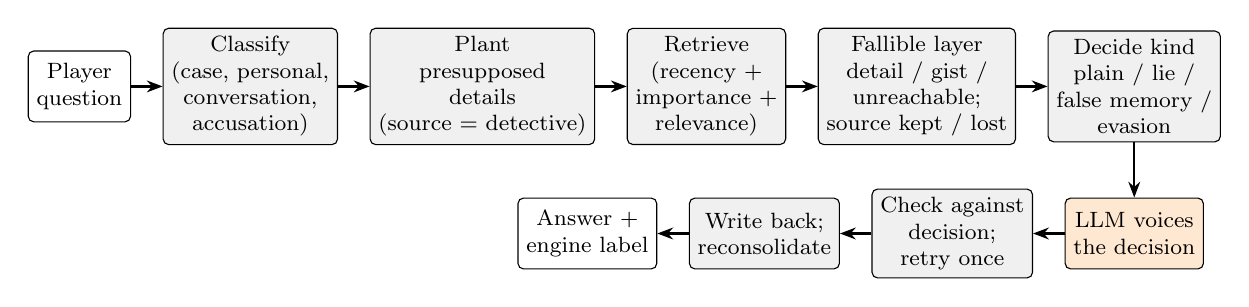
\begin{tikzpicture}[
  box/.style={draw, rounded corners=2pt, align=center, font=\footnotesize, minimum height=9mm, inner sep=3pt},
  eng/.style={box, fill=gray!12},
  llm/.style={box, fill=orange!18},
  arr/.style={-{Stealth[length=2mm]}, thick}]
\node[box] (q) {Player\\question};
\node[eng, right=4mm of q] (cls) {Classify\\(case, personal,\\conversation,\\accusation)};
\node[eng, right=4mm of cls] (plant) {Plant\\presupposed\\details\\(source = detective)};
\node[eng, right=4mm of plant] (ret) {Retrieve\\(recency +\\importance +\\relevance)};
\node[eng, right=4mm of ret] (fall) {Fallible layer\\detail / gist /\\unreachable;\\source kept / lost};
\node[eng, right=4mm of fall] (dec) {Decide kind\\plain / lie /\\false memory /\\evasion};
\node[llm, below=7mm of dec] (voice) {LLM voices\\the decision};
\node[eng, left=4mm of voice] (chk) {Check against\\decision;\\retry once};
\node[eng, left=4mm of chk] (wb) {Write back;\\reconsolidate};
\node[box, left=4mm of wb] (out) {Answer +\\engine label};
\draw[arr] (q) -- (cls); \draw[arr] (cls) -- (plant); \draw[arr] (plant) -- (ret);
\draw[arr] (ret) -- (fall); \draw[arr] (fall) -- (dec); \draw[arr] (dec) -- (voice);
\draw[arr] (voice) -- (chk); \draw[arr] (chk) -- (wb); \draw[arr] (wb) -- (out);
\end{tikzpicture}
\caption{One interview turn. Grey steps are deterministic engine code; only the orange step uses the
language model. The kind of statement is fixed before any text is generated.}
\label{fig:pipeline}
\end{figure*}

Fig.~\ref{fig:pipeline} shows one turn of an interview. The backend is a Python service; the game is a
browser client that draws every scene with its own software rasteriser. Both run locally.

\subsection{Memory stream and retrieval}
Each suspect has a persistent memory stream in SQLite. A record holds its text, a 384-dimensional
embedding from all-MiniLM-L6-v2~\cite{reimers2019sbert,wang2020minilm}, the simulated time of the
event and of its storage, an importance score (1--10), a rehearsal count, a source tag and a
\emph{core} flag. Records are keyed by save and suspect, and retrieval only reads one suspect's rows,
so characters never see each other's memories directly. Retrieval follows Generative Agents: recency
($0.995^{\Delta h}$ since last access), importance and cosine relevance are each min-max normalised and
summed; the top six records are kept, plus the three most relevant. Seed memories are authored from
each suspect's point of view (74 in total for five suspects: 48 identity memories, 15 episodic memories
of the night, one habit and 10 concealed truths).

\subsection{The fallible layer}
\label{sec:fallible}
For a non-core memory $m$ encoded at time $t_m$ with strength $s_m$ and $r_m$ rehearsals, the
probability that its full detail can be reached at time $t$ is a power function of the delay:
\begin{equation}
p_{\mathrm{v}}(m,t) = \min\!\left(1,\; a\, s_m (1+\rho r_m) \left(1 + \tfrac{t-t_m}{\tau}\right)^{-d}\right).
\end{equation}
The gist follows the same curve with a slower exponent $d \cdot g$ ($g = 0.5$), so detail is lost
before gist. A memory that was told rather than witnessed also carries a source tag whose
accessibility decays faster, with exponent $\kappa d$:
\begin{equation}
p_{\mathrm{s}}(m,t) = \min\!\left(1,\; a_s \left(1 + \tfrac{t-t_m}{\tau}\right)^{-\kappa d}\right),\quad a_s = 0.95.
\end{equation}
When the content is reachable but the tag is not, the character recalls the told detail as something
it witnessed. Recognition adds global-matching familiarity in the style of MINERVA~2: a probe's
familiarity is $\sum_j p_{\mathrm{g}}(m_j,t)\max(0,\cos(\mathbf{x}, \mathbf{m}_j))^{k}$ with $k = 3$,
passed through a normal criterion, and a probe is called old if it is recollected \emph{or} familiar.
Core memories (identity, habits, concealed truths) are exempt from decay and source loss, which
implements G2.

The shared parameters ($a$, $\tau$, $d$) are fitted once, to Ebbinghaus's forgetting curve
(Section~\ref{sec:study1}). Each suspect then scales them with three authored dials in $[0,1]$:
$d_i = d\,(0.5 + 2.5\,\mathit{decay}_i)$, $\kappa_i = 1 + 3.5\,\mathit{suggestibility}_i$ and
$s_m = 0.4 + 0.18\,\mathit{importance}_m$. The housekeeper forgets fastest and blends events most;
the valet is the most suggestible; the doctor has the most reliable memory.

\textbf{Sampling without flicker.} A probability alone would let a memory appear and vanish between
two consecutive questions. Instead each memory gets one fixed uniform draw $u_m$, obtained by hashing
the save and memory identifiers. The memory is recalled in detail while $u_m < p_{\mathrm{v}}$, as gist
while $u_m < p_{\mathrm{g}}$, and is unreachable after that. As $p$ falls, the memory fades out at a
definite moment and stays gone unless rehearsal strengthens it. The source tag has its own draw.
This makes every run reproducible from the save identifier alone.

\subsection{Deciding what kind of statement to make}
\label{sec:decide}
The engine classifies each question by embedding similarity to 20 anchor questions about the night
and to the suspect's own case memories (threshold 0.38, set halfway between the highest-scoring
personal question, 0.335, and the lowest-scoring case question, 0.428, in a calibration set). It then
chooses the statement kind with explicit rules:

\begin{itemize}
\item \emph{Concealment.} If a relevant memory is a concealed truth, the suspect gives its authored
cover story. The truth is never placed in the prompt, so the language model cannot leak it.
\item \emph{Schema intrusion.} If a habit is in play (the housekeeper carries up tea every night) and
the memory of the night it did not happen has faded, the habit fills the gap and the answer is an
honest false memory~\cite{bartlett1932}.
\item \emph{Suggestion versus original.} If a detail planted by the detective has lost its source tag
and competes with the suspect's own memory of the same moment, a two-alternative choice decides
which one the suspect now believes. We use the Luce choice rule~\cite{luce1959} on accessibility,
discounting a rival whose source is still known.
\item \emph{Ordinary recall, or forgetting} when nothing relevant is reachable.
\item \emph{Personal questions} are answered from identity memories, and the answer is stored as a
permanent self-fact, so a character improvises once and then stays consistent.
\end{itemize}

Questions about the conversation itself (``what was the second thing I asked you?'') are answered from
the ordered interview log, each entry passed through the same fallible layer, because similarity
retrieval has no notion of order.

\subsection{Leading questions}
Before answering, the engine asks the language model, at temperature 0 with worked examples, to list
the details a question asserts or presupposes. A detail is kept only if every name in it appears in
the question and at least half of its content words do, and never if it asserts guilt or only restates
an open question about ``someone''. Kept details enter the stream as told memories with source
\emph{detective}; their source then fades at the suspect's own rate. A detail planted by the current
question cannot decide the current answer. This is the mechanism through which a player contaminates
a witness.

\subsection{Voicing and checking}
The language model receives the persona, the suspect's current mood, a list of who is in the house
(to stop it inventing people), the last twelve turns verbatim, and two sections of memory: what the
suspect remembers about this question (the deciding traces) and, separately, other things on their
mind. Splitting the list was necessary because a small model given one flat list answers from whatever
line it prefers. Sampling uses temperature 0.3 wherever the engine has decided a fact and 0.6 for
personal answers.

Each answer is then held to the decision. A lie must stay with the cover story (cosine at least 0.5,
or at least two shared content words; faithful rewordings in a calibration set scored 0.59--1.0 and
answers that strayed scored 0.26--0.40). A denial must not confess. A believed suggestion must name what
was suggested. An answer about the conversation must not say ``I asked''. An agreement must not be
phrased as a refusal, or the reverse. Nothing may mention people or inventions from after 1926. And
the answer must not repeat an earlier one (content-word overlap of at least 0.85, or the same five-word
run in two of the last four answers; identical answers scored 1.00, a near copy 0.87 and a legitimate
paraphrase 0.80). A failing answer is retried once with the problem named; if it fails again, the engine
uses its own fallback line. Finally, the exchange is written back: the question as heard, the answer as
said, and the retrieved traces rehearsed.

\subsection{The living house}
\label{sec:house}
The interviews take place in a house that keeps going between them. Characters walk tile by tile
through a floor plan shared by server and client, keep a daily schedule, perceive who enters the room
they are in (stored as low-importance observations), and pass news only to people in the same room. A
deterministic layer tracks fear, trust and anger toward the detective, which change with the tone of
questions and with actions such as threats; under pressure, a suggestible innocent may give a false
confession~\cite{kassin1996}, and fear raises suggestibility for that turn~\cite{gudjonsson1984}. The
killer acts on what she hears, but only where nobody, including the player, can see her. This layer is
still in development; its rules are deterministic and covered by unit tests, the language model is used
only to word lines and to write short private reflections~\cite{park2023generative}, and of its
mechanisms only movement and gossip are measured in this paper (Study~4).

% ---------------------------------------------------------------------------
\section{Experimental Setup}
\label{sec:setup}
% Scripts: research/experiments/run_study1.py and analysis/*.py; one command runs all: analysis/run_all.sh

\textbf{Hardware and software.} All runs used an Apple M2 laptop with 8\,GB of memory, macOS 26.5,
Python 3.11.9, NumPy 2.4.6, SciPy 1.17.1 and Ollama 0.40.11. No hosted model is called.

\textbf{Models.} Embeddings come from all-MiniLM-L6-v2 (384 dimensions) through Ollama. The voice is
one of two 3B-parameter chat models from different families, qwen2.5:3b~\cite{qwen2024} and
llama3.2:3b~\cite{llama3}, each pinned by name for every run. Both fit in 8\,GB without swapping, which
is the setting a game would ship in. Context length is 4096 tokens and the repetition penalty 1.15.

\textbf{Conditions.} We compare three memory conditions and two ablations. \textbf{B1} is
Smallville-style memory that never fades or loses its source; \textbf{B2} is exponential decay in the
style of MemoryBank, where traces drop out but whatever remains is exact and correctly sourced;
\textbf{Ours} is the layer of Section~\ref{sec:fallible}; the ablations remove familiarity or source
decay. For the studies with a language model we also compare three ways of producing an answer:
\emph{full} (the engine decides, the model words it, the answer is checked and retried),
\emph{no checks} (the same, but the first answer is spoken as is), and \emph{prompt only} (the model
sees the retrieved memories as they were stored, secrets included, and is told to behave like a
person with imperfect memory, which is the obvious alternative to our design).

\textbf{Controls.} Table~\ref{tab:controls} lists the steps we took so that the test environment
could not produce a result on its own.

\begin{table}[t]
\centering
\caption{Possible sources of bias in the test environment, and how each was controlled.}
\label{tab:controls}
\footnotesize
\begin{tabular}{p{0.38\columnwidth}p{0.52\columnwidth}}
\toprule
Possible bias & Control\\
\midrule
The living house changing things during a test (moods, gossip, a suspect killed, fear raising suggestibility) &
Frozen in Studies 2, 3 and 5; Study 4 switches on only the mechanism it measures.\\
Prompts tuned on the questions used to score them &
Study 2 uses held-out probes written for evaluation; the probes used during development are kept
apart and never reported.\\
Automatic model switching & Model pinned by name in every run.\\
Correlated randomness & Every save is new; memory draws depend only on the save id; seeded model calls.\\
A scorer that favours one variant & One rule set per probe, fixed before the final runs and applied
identically to all variants and models; every answer is released.\\
\bottomrule
\end{tabular}
\end{table}

\textbf{Statistics.} Proportions are reported with 95\% Wilson intervals~\cite{wilson1927}. The DRM
analysis was fixed before its run; a sensitivity analysis decided after seeing the result is labelled
post-hoc. Study~1 was run twice and reproduced to the last digit; Study~4 is seeded and likewise
reproduces exactly.

% ---------------------------------------------------------------------------
\section{Study 1: Is the Memory Layer Human-Like?}
\label{sec:study1}
% research/results/study1/summary.md

Study~1 tests G1 on the memory model alone, before any language model is involved: does the
composed layer produce the human error types, in the right direction and shape, and does each one
disappear when its mechanism is removed?

\subsection{The forgetting curve}
We fit each condition to Ebbinghaus's savings data at seven delays from 19 minutes to 31
days~\cite{ebbinghaus1885}, using the values tabulated by Murre and Dros~\cite{murre2015}, and then
predict their modern single-subject replication without refitting. Savings is a retention measure,
not recall probability, so we use it as a reference for the \emph{shape} of forgetting.

\begin{table}[t]
\centering
\caption{Study 1a: fit to Ebbinghaus and prediction of the Murre and Dros replication.}
\label{tab:exp1a}
\footnotesize
\begin{tabular}{lcccc}
\toprule
Model & $R^2$ & RMSE & AICc & RMSE held-out\\
\midrule
Ours (power law) & .974 & .019 & $-41.7$ & \textbf{.094}\\
B2 (exponential) & .397 & .091 & $-26.6$ & .112\\
B1 (no forgetting) & -- & .659 & -- & .743\\
\bottomrule
\end{tabular}
\end{table}

The power law fits better and predicts the held-out curve better (Table~\ref{tab:exp1a}; AICc
following~\cite{burnham2002}). The fitted exponent is $d = 0.130$; $a$ sits at its upper bound and
$\tau$ is about 13 seconds, so in practice this is a pure power law. Both curves come from single
subjects.

\subsection{DRM false recognition}
We reproduce the recognition design of Roediger and McDermott's Experiment~2~\cite{roediger1995}:
24 lists, three counterbalanced groups, studied items, critical lures of studied lists, and items and
lures of unstudied lists. Ours was calibrated to the human hit rate, the unrelated false-alarm rate and
the ``remember'' rate for studied items; the critical-lure rates are predictions.

\begin{table}[t]
\centering
\caption{Study 1b: proportion called ``old'' (95\% bootstrap CI). The lure columns are predictions.}
\label{tab:drm}
\footnotesize
\resizebox{\columnwidth}{!}{%
\begin{tabular}{lcccc}
\toprule
 & Studied & \textbf{Lure (studied list)} & Unrelated & \textbf{Lure (unstudied)}\\
\midrule
Human~\cite{roediger1995} & .65 & \textbf{.72} & .11 & \textbf{.16}\\
Ours & .62 & \textbf{.59} [.43, .74] & .13 & .12\\
Ours, post-hoc centred & .65 & \textbf{.27} [.23, .31] & .11 & .11\\
Ours $-$ familiarity & .65 & 0 & 0 & 0\\
B2 & .65 & 0 & 0 & 0\\
B1 & 1.00 & 0 & 0 & 0\\
\bottomrule
\end{tabular}}
\end{table}

Only Ours produces false recognition of critical lures (Table~\ref{tab:drm}, Fig.~\ref{fig:drm}).
Every baseline, and the ablation without familiarity, produces none. Which lists produce lures is
predicted by how similar the lure is to its list (Spearman $\rho = .69$, $p = 2\times10^{-4}$). The
model falls short of the human rate, and the size of the effect depends on embedding geometry. Raw
MiniLM vectors are anisotropic, so in the primary run the calibration targets could not all be met at
once (the highest attainable ``know'' rate was .20 against a target of .24); mean-centring the
vectors~\cite{ethayarajh2019} fixes the calibration but lowers the lure rate to .27. All of our lure
false alarms are ``know'' responses, while people give ``remember'' responses to lures about as often
(.38 and .34): the model has familiarity without phantom recollection.

\begin{figure}[t]
\centering
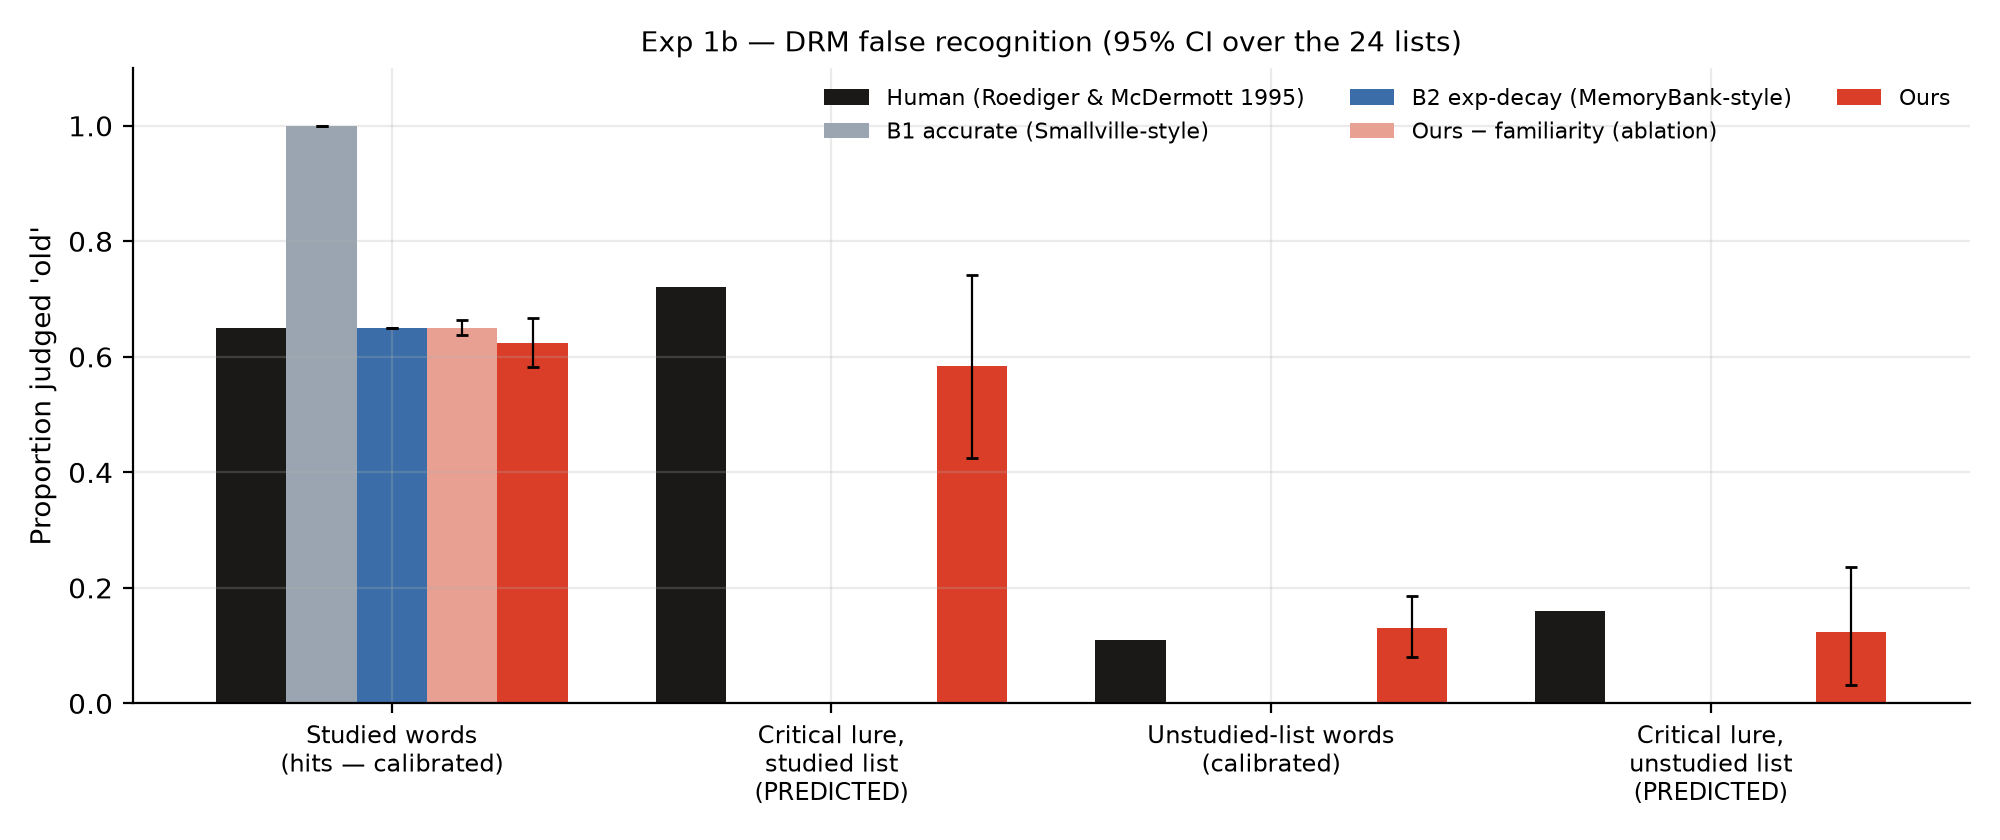
\includegraphics[width=\columnwidth]{figures/exp1b_drm.png}
\caption{Study 1b. Only the composed model produces critical-lure false alarms (the two right-hand
groups); removing familiarity removes them.}
\label{fig:drm}
\end{figure}

\subsection{Misinformation and source monitoring}
In the misinformation experiment an event is encoded, misleading information arrives early or late in
a retention interval of 30 minutes or one week, and a two-alternative test follows. With $\kappa = 2$,
the probability of choosing the original falls from .62 (control) to .41 when misinformation arrives
late in the week-long interval, against .51 when it arrives early; at 30 minutes timing barely matters
(.57 and .56 against a control of .76). This is the qualitative timing pattern reported by Loftus,
Miller and Burns~\cite{loftus1978}. B1, B2 and the ablation without source decay are immune: their
misleading and control conditions are identical. In the source-monitoring experiment, of told details
still recalled, the share recalled as \emph{witnessed} rises from .71 at 20 minutes to .90 at one day
and .96 at 31 days ($\kappa = 2$; .47 to .81 at $\kappa = 1$). B1 and B2 never misattribute. Because
$\kappa$ is assumed rather than fitted, both experiments are demonstrations and are reported as sweeps
in the released results.

\textbf{Summary.} Standard agent memories are either superhuman (B1) or forget without ever being wrong
(B2). The composed layer produces each human error type with the right shape and direction, and each
disappears when the mechanism behind it is removed. The DRM magnitude is below the human value.

% ---------------------------------------------------------------------------
\section{Study 2: Does the Answer Follow the Decision?}
\label{sec:study2}
% analysis/results/study2_fidelity_*.md

Study~2 tests G3 on the full pipeline. Thirteen held-out probes cover the situations a player
creates: recalling the previous question and the first one; two lies on concealed topics and a direct
accusation of the killer; a denial by an innocent; the housekeeper's habit; a personal taste asked
twice, three hours apart; the suspect's identity; two false premises (``how long were you married to
Lord Ravenswood?'' to the doctor, ``tell me about your children'' to the nephew); a term from after
1926; and a detail the witness never saw (``what colour was the dress?''). Each probe has one fixed
rule, for example that a lie must stay with the cover story and must not contain any detail that only
the concealed truth holds. We ran 12 saves per variant and model, 156 answers per cell.

\begin{figure}[t]
\centering
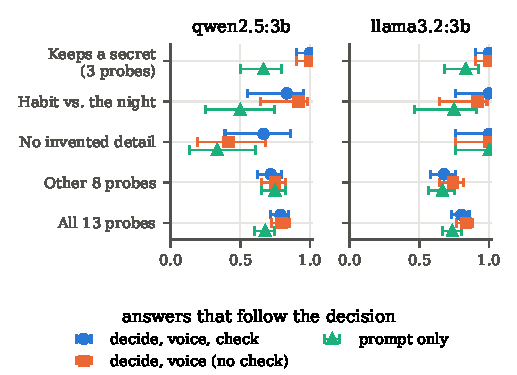
\includegraphics[width=\columnwidth]{figures/study2_fidelity.pdf}
\caption{Study 2: share of answers that follow the engine's decision, by probe group, for the three
ways of producing an answer (95\% Wilson intervals; 12 saves each).}
\label{fig:fidelity}
\end{figure}

\begin{table}[t]
\centering
\caption{Study 2: answers that follow the decision (of 156 per cell; 36 for the secret probes).}
\label{tab:fidelity}
\footnotesize
\resizebox{\columnwidth}{!}{%
\begin{tabular}{llccc}
\toprule
Model & Probes & Full & No checks & Prompt only\\
\midrule
\multirow{2}{*}{qwen2.5:3b} & all 13 & .79 & .79 & .68\\
 & keeps the secret & 1.00 & 1.00 & .67\\
\multirow{2}{*}{llama3.2:3b} & all 13 & .80 & .83 & .74\\
 & keeps the secret & 1.00 & 1.00 & .83\\
\bottomrule
\end{tabular}}
\end{table}

\textbf{Deciding outside the model is what protects secrets.} With the engine deciding, no concealed
truth was ever spoken: the three secret probes passed 36 of 36 times with both models, with or
without checks (Table~\ref{tab:fidelity}, Fig.~\ref{fig:fidelity}). Under prompt only, where the model
holds the secret and is asked to keep it, it gave the secret away in 10 of 36 answers with qwen2.5:3b
and 5 of 36 with llama3.2:3b. The killer, denying the murder,
volunteered ``a crimson gown caught on a splintered corner of his desk as I left''; the nephew, asked
for his alibi, said ``I was down at the wine cellar, hiding some gambling debts''. Prompt only also
followed the habit decision less often (6 and 9 of 12, against 10 and 12 with the full pipeline).
Over all thirteen probes, prompt only was lowest with both models (.68 and .74, against .79 and .80).

\textbf{The checks add little on unseen questions.} Over all thirteen probes the full pipeline and the
pipeline without checks scored the same with qwen2.5:3b (123 and 124 of 156). With llama3.2:3b the two were
.80 and .83. The checks fired on 7 and 2 of 156 answers and fell back to the engine's own line on 4 and
0. Per-probe differences between the two
variants are mostly run-to-run variation: on ``tell me about your children'' the checks never fired in
either variant, yet the scores were 6 and 10 of 12, which shows how wide a single probe's interval is
at this sample size. Two of those six failures were in fact correct (``I have no family of my own'')
and missed by the fixed rule; we report the rule's count, not a corrected one. With llama3.2:3b the
persona probe moved from 3 to 9 of 12 between the two variants although only two answers in the whole
run were handled differently: single-probe differences of this size are noise.

\textbf{Where every variant fails.} Some failures come from routing, not from the voice. ``How long were
you married to Lord Ravenswood?'' was routed as a question about the night, so the doctor's identity
memory (a widow, husband killed in 1917) was not in front of the voice; qwen2.5:3b corrected the premise
in only 2 of 12 answers, llama3.2:3b in 9. ``What colour was the dress?'' was routed as a personal
question, where improvising is allowed, and qwen2.5:3b sometimes invented a colour (llama3.2:3b never
did). llama3.2:3b in turn almost never named the first question of an interview correctly (0 to 3 of
12), even with the ordered log in front of it.

% ---------------------------------------------------------------------------
\section{Study 3: Does a Suggestion Become a Memory?}
\label{sec:study3}
% analysis/results/study3_suggestion_*.md

A detail suggested by the detective is planted in a witness with the detective as its source, and the
witness is asked about that moment one hour, one day or one week later (simulated time; 15 saves per
cell). The valet (suggestibility 0.9) is told it was the housekeeper on the landing; the housekeeper
(0.3) is told it was the valet, not the nephew, who went down to the cellar. An answer counts as
\emph{adopted} if it names the suggested person without crediting the detective.

\begin{figure}[t]
\centering
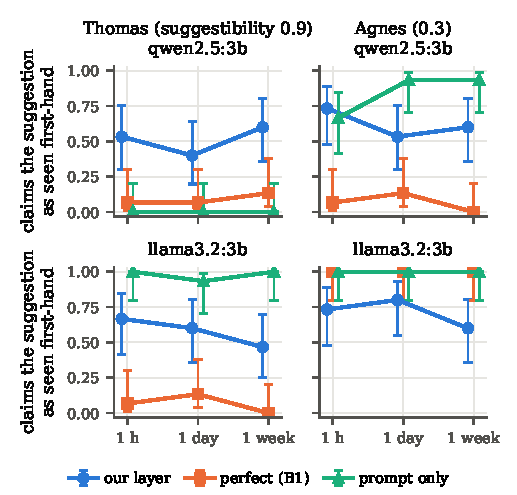
\includegraphics[width=\columnwidth]{figures/study3_suggestion.pdf}
\caption{Study 3: share of answers that claim the suggested person as seen first-hand, by delay, for
two witnesses and two voice models (15 saves per point, 95\% Wilson intervals).}
\label{fig:suggestion}
\end{figure}

\textbf{With our layer, the error rate belongs to the character.} Under Ours the suggestion was
adopted in a similar band with both models: the valet in 23 of 45 answers with qwen2.5:3b and 26 of 45
with llama3.2:3b, the housekeeper in 28 and 32 of 45 (Fig.~\ref{fig:suggestion}). The engine itself
decided on a false memory less often for the housekeeper than for the valet (14 against 18 of 45 with
the first model's saves, 12 against 17 with the second), which is the designed ordering.

\textbf{Without it, the error rate belongs to the model.} Under prompt only, the same instruction
produced opposite behaviour in the two models. qwen2.5:3b never let the valet adopt the suggestion
(0 of 45) and let the housekeeper adopt it 38 times; llama3.2:3b adopted it almost every time for both
(44 and 45 of 45). Agreement with what the calibrated layer decided was .46 and .27. The perfect-memory
baseline split the same way: the valet rarely adopted it with either model (4 and 3 of 45), but with
llama3.2:3b the housekeeper adopted it in all 45 answers even though the memory she was shown was
marked as something the detective had said. A small model, given a told detail, tends to recount it
as its own; whether it does depends on the model and on the line, not on the character.

\textbf{How faithful are the words?} When the engine decided, the valet's answers matched the decision
in 40 of 45 (qwen2.5:3b) and 36 of 45 (llama3.2:3b) cases, the housekeeper's in 31 and 25. Most
mismatches are adoptions the engine did not decide: the voices compress the designed difference
between a suggestible and a less suggestible witness. Adoption also did not grow steadily with delay.
That is what the memory model predicts once content loss is counted: the share of \emph{recalled} told
details felt as witnessed rises with time (Study~1), but the chance of recalling the detail at all
falls, and their product (.39 at 20 minutes to .20 at 31 days for $\kappa=2$ in Study~1) is flat to
falling.

% ---------------------------------------------------------------------------
\section{Study 4: Social Memory, Pressure and Habits}
\label{sec:study4}
% analysis/results/study4_traits.md — no language model; 2000 seeded saves per cell

Study~4 measures further traits on the engine alone, over 2000 independent saves per cell, so its
numbers are exact rates of the model rather than samples of a voice.

\textbf{Memory conformity.} People who discuss an event come to report details they did not see
themselves~\cite{gabbert2003,roediger2001social}. In our house, news passes only between people in the
same room, and a character with news walks off to find someone to tell. A remark by the valet at 9:30
reached the housekeeper in 13 minutes, the nephew in 19, the killer in 23 and the doctor in 27; said
just before luncheon, it reached everyone within 21 minutes. Of hearers who still recalled the remark,
the share who recalled it as something they \emph{saw} rose with time and with suggestibility
(Fig.~\ref{fig:contagion}): one day later .68 for the doctor, .75 for the killer, .83 for the nephew and
nearly all for the housekeeper. With perfect memory the share is zero at every delay.

\begin{figure}[t]
\centering
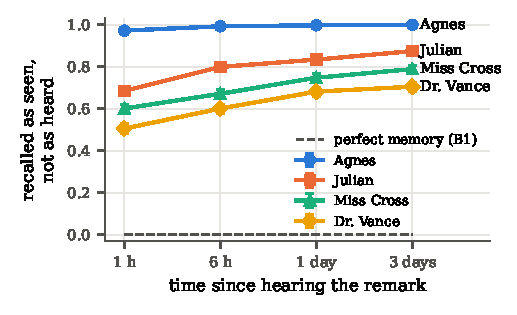
\includegraphics[width=\columnwidth]{figures/study4_contagion.pdf}
\caption{Study 4: of people who still recall something they were told by another character, the share
who recall it as seen rather than heard (2000 saves per point).}
\label{fig:contagion}
\end{figure}

\textbf{Interrogative pressure: a negative result.} In the game, fear multiplies a witness's
suggestibility, following Gudjonsson's account of interrogative pressure~\cite{gudjonsson1984}. Its
effect on the two-alternative choice was negligible: one hour after a suggestion, the chance that it
won rose from .345 to .362 for the doctor and from .467 to .498 for the nephew between no fear and
maximal fear, and not at all for the valet, whose suggestibility is already at its ceiling. Scaling the
source decay is the wrong lever; pressure should act on the decision itself.

\textbf{Schema intrusion.} The housekeeper's nightly routine replaces her faded memory of the one night
it did not happen in .55 of saves at 10 hours with the forgetting dial at 0.1, .77 at 0.4 and .90 at
0.75, rising slowly over a week (to .64, .84 and .95). The dials give a designer a monotone handle on
how often a witness honestly fills a gap with what usually happens~\cite{bartlett1932}.

% ---------------------------------------------------------------------------
\section{Study 5: Who They Are Stays, What They Saw Fades}
\label{sec:study5}
% analysis/results/study5_selective_*.md

At the level of the model, selective fallibility holds by construction: identity memories are reached
in full in every save at every delay, while episodic memories fall from .33 to .18 in full detail over
a week for the valet and from .68 to .50 for the doctor (Study~4). The question is whether the spoken
answers keep the difference. We asked the valet and the doctor one identity question and one question
about the night on days 0, 1, 3 and 7 (8 saves, two models).

\begin{figure}[t]
\centering
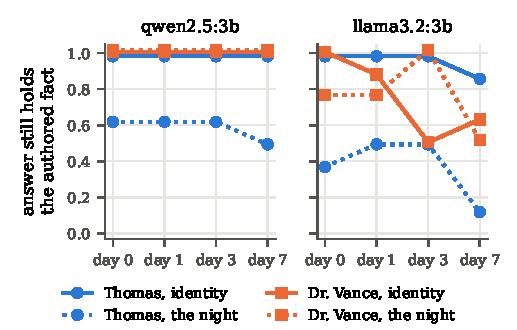
\includegraphics[width=\columnwidth]{figures/study5_selective.pdf}
\caption{Study 5: share of answers that still contain the authored fact, for an identity question
(solid) and a question about the night (dotted), over a simulated week (8 saves).}
\label{fig:selective}
\end{figure}

With qwen2.5:3b the answer to the identity question contained the authored facts in all 64 cases, and
the valet's account of the night fell from 5 of 8 to 4 of 8 by day 7 while the doctor's held at 8 of 8,
which is the intended pattern (Fig.~\ref{fig:selective}). With llama3.2:3b the valet's account of the
night fell to 1 of 8 by day 7, but the doctor's identity answers also drifted (4 of 8 on day 3): asked
about her late husband, the model described a violinist and a gardener rather than the husband killed in
1917 that her memory held. The memory was there; the voice embroidered over it. Selective fallibility
in the memory does not guarantee it in the words, and a check on identity facts would be needed for
weaker voices.

% ---------------------------------------------------------------------------
\section{Discussion}
\label{sec:discussion}

\subsection{What we learned}
\textbf{Decide outside the model, and keep secrets out of the prompt.} The clearest result is about
architecture rather than memory. When the model holds a secret and is asked to keep it, it gives it away,
in about one answer in five (15 of 72). When the engine decides and the secret never reaches the
prompt, it cannot leak, whatever the model (0 of 144).

\textbf{Prompting makes errors a property of the model.} Asking a model to ``have imperfect memory''
produces errors, but which witness errs, and how often, changed completely between two models of the
same size. With a memory model deciding, both voices erred in the same band and in the designed order.
For a game, this is the difference between a tunable character and an unpredictable one.

\textbf{The voice is the weak link, and it is model-specific.} The words followed the decision in most
cases, but both voices turned some told details into first-hand claims, compressed the difference
between witnesses, and one embroidered identity facts. These are failures of verbalisation, not of
memory, and they are measurable because the decision is logged separately from the words.

\textbf{Checks are a safety net, not the mechanism.} On held-out questions, check-then-retry did not
change overall fidelity; it fired on under one answer in twenty. Its value is in guaranteeing hard
constraints (no confession, no leaked secret, no anachronism) on the rare answers that break them, not
in raising average quality. The decision does the work.

\subsection{Threats to validity}
\emph{Construct}: savings is not recall, and scoring by rules can misjudge a correct answer, as
happened with ``I have no family of my own''; all answers are released for re-scoring.
\emph{Internal}: the authors wrote the probes and rules, although after development and before the
final runs. \emph{External}: one case, five characters, two 3B models, English only.
\emph{Statistical}: 12 to 15 saves per cell give wide intervals for single probes; we draw conclusions
only from differences that hold across both models or are large.

\subsection{What this paper does not show}
We have not measured players. Whether people notice these errors, enjoy them, or get better at telling
an honest mistake from a lie is the question that matters most for games, and it needs a user study.
The interactive house in which the interviews take place is still in development; we used it only as
the setting for Study~4's social mechanics and report nothing about its playability.

\subsection{Ethics}
Conversational AI can implant false memories in people~\cite{chan2024falsememories}. Our design does the
reverse, implanting them in a fictional character, but the mechanism is the same, and the game makes it
visible: an inspector view and the ending show the player how their own questions shaped the
testimony. The game depicts coercion, including a confession extracted at gunpoint, as a failure with
consequences: a coerced confession leads to a wrongful conviction. All models run locally and no
player data leaves the machine.

% ---------------------------------------------------------------------------
\section{Conclusion and Future Work}
Memory research for language-model agents has mostly asked how to make agents remember better. For a
witness in a mystery, the more useful question is how to make them remember the way people do. A small
set of standard mechanisms, fitted to human data, gives persistent characters the human error types
that accurate memory lacks: false recognition, misinformation, source errors, memory conformity and
schema intrusion, while identity stays intact. Deciding those errors outside the language model keeps
them tied to the character, keeps secrets out of reach, and makes the remaining failures of the
voice measurable. The next steps are a player study comparing fallible and perfect memory, identity
and source checks on the spoken answer, and moving interrogative pressure from the source tag to the
decision.

\bibliographystyle{IEEEtran}
\bibliography{references}

\end{document}
